\documentclass[a4paper]{report}
\usepackage[utf8]{inputenc}
\usepackage[T1]{fontenc}
\usepackage[francais]{babel}
\usepackage{listings}
\usepackage{color}
\usepackage{listingsutf8}
\usepackage[pdftex]{graphicx}
\usepackage{float}
\usepackage{titlesec}
\usepackage{fullpage}
\usepackage{pdfpages}
\usepackage[section]{placeins}
\usepackage{pdflscape}
\usepackage{amsmath}
\usepackage{mathtools}
\usepackage{hyperref}
\usepackage{enumitem}
\usepackage{graphicx}

\usepackage{array,multirow,makecell}
\setcellgapes{1pt}
\makegapedcells
\usepackage[table]{xcolor}

\definecolor{navy}{rgb}{0,0.4,0.75}
\definecolor{grey}{rgb}{0.4,0.4,0.4}
\definecolor{blueTitle}{RGB}{10, 45, 130}
\titleformat{\chapter}{\color{blue}\normalfont\huge\bfseries}{\thechapter}{1em}{} 
\newcommand{\HRule}{\rule{\linewidth}{0.5mm}}
\newcolumntype{C}[1]{>{\centering\arraybackslash }b{#1}}

\hypersetup{                    
	colorlinks=true,	% colorise les liens
	breaklinks=true,    % permet les retours à la ligne pour les liens trop longs
	urlcolor= navy,		% couleur des hyperliens
	linkcolor= black,    % couleur des liens internes aux documents (index, figures, tableaux, equations,...)
	citecolor= navy      % couleur des liens vers les references bibliographiques
}

\lstset{backgroundcolor=\color{white},   
	basicstyle=\footnotesize,        
	breakatwhitespace=false,        
	breaklines=true,               
	captionpos=b,                
	commentstyle=\color{grey},    
	extendedchars=true,         
	frame=false,               
	keepspaces=true,          
	keywordstyle=\color{blue}, 
	language=C++,             
	literate=
	{²}{{\textsuperscript{2}}}1
	{⁴}{{\textsuperscript{4}}}1
	{⁶}{{\textsuperscript{6}}}1
	{⁸}{{\textsuperscript{8}}}1
	{€}{{\euro{}}}1
	{é}{{\'e}}1
	{è}{{\`{e}}}1
	{ê}{{\^{e}}}1
	{ë}{{\¨{e}}}1
	{É}{{\'{E}}}1
	{Ê}{{\^{E}}}1
	{û}{{\^{u}}}1
	{ù}{{\`{u}}}1
	{â}{{\^{a}}}1
	{à}{{\`{a}}}1
	{á}{{\'{a}}}1
	{ã}{{\~{a}}}1
	{Á}{{\'{A}}}1
	{Â}{{\^{A}}}1
	{Ã}{{\~{A}}}1
	{ç}{{\c{c}}}1 
	{Ç}{{\c{C}}}1
	{õ}{{\~{o}}}1
	{ó}{{\'{o}}}1
	{ô}{{\^{o}}}1
	{Õ}{{\~{O}}}1
	{Ó}{{\'{O}}}1
	{Ô}{{\^{O}}}1
	{î}{{\^{i}}}1
	{Î}{{\^{I}}}1
	{í}{{\'{i}}}1
	{Í}{{\~{Í}}}1,
	numbers=left,            
	numbersep=5pt,          
	numberstyle=\tiny\color{black},
	rulecolor=\color{black},      
	showspaces=false,            
	showstringspaces=false,     
	showtabs=false,            
	stepnumber=1,             
	stringstyle=\color{red}, 
	tabsize=4,              
	title=\lstname,        
}

\title{ENSICAEN - 2A Spécialité Informatique\\Projet 2A}
\author{\textsc{Vimont} Ludovic \& \textsc{Kotulski} Guillaume}
\date{\today}
\makeatletter

\begin{document}

\begin{titlepage}
	\begin{center}
		\vspace*{\fill}
		\textsc{\Large \@title } 
		\HRule
		\vspace{1.5cm}
		\begin{center}
			
\includegraphics[width=0.6\textwidth]{data/logo.png}
		\end{center}
		\vspace{1.5cm}
		\HRule \\
		\Large{Reconnaissance faciale : anti-fake}\\

		\large{\@author} \\
		\vspace*{\fill}

		\bsc{Promo 2016} \\
		\@date
	\end{center}
\end{titlepage}

\chapter*{Remerciements}
\bsc{Faye} Ndiaga 
\bsc{Schwartzmann} Jean-Jacques


\setcounter{tocdepth}{4}
\renewcommand{\contentsname}{Sommaire} 
\tableofcontents

\chapter{Introduction}
\section{Contexte}

Dans le cadre des cours de l'ENSICAEN, nous devions réaliser un projet de deuxième année. Nous avons choisi de prendre le projet reconnaissance faciale anti-fake proposé
par M. \bsc{Schwartzmann} Jean-Jacques. 

\section{Objectifs}

L'objectif du projet est la réalisation d'un moyen d'authentification par reconnaissance facile grâce à l'utilisation d'une capture vidéo. En effet, actuellement ce genre d'applications sont facilement 
attaquables. Prenons l'exemple d'un smartphone qui se déverrouille grâce à ce moyen. Il suffit pour un attaquant de disposer de la photo de la victime pour contourner la protection. Ce projet consiste donc 
à utiliser une capture vidéo et être capable de différencier un humain d'une photo grâce à cette enregistrement. Afin de réaliser cette différenciation, nous devions baser notre travail sur une \href{http://people.csail.mit.edu/mrub/papers/vidmag.pdf}{recherche} du MIT. Enfin, nous devons intégrer notre résultat dans une application android de reconnaissance faciale forunie par le \href{https://www.greyc.fr/}{GREYC}.

\section{Contraintes}

La seule contrainte dont nous disposions était le temps de reconnaissance de la personne, en effet pour l'application android au-dessus de 4 secondes cela était beaucoup trop long, d'un point de vue 
utilisateur. 


\chapter{Développement}
\section{Outils mis en place}

Afin de mener à bien notre projet, nous avons utilisé différents outils de gestion de projets :

\begin{itemize}
	\item Pour permettre le suivi du projet, nous avons mis en ligne un site web, ce dernier utilise le CMS\footnote{Content Management System (ou système de gestion de contenu)} Wordpress : \url{http://www.ecole.ensicaen.fr/~lvimont/}

		\begin{figure}[h!]
			\centering
			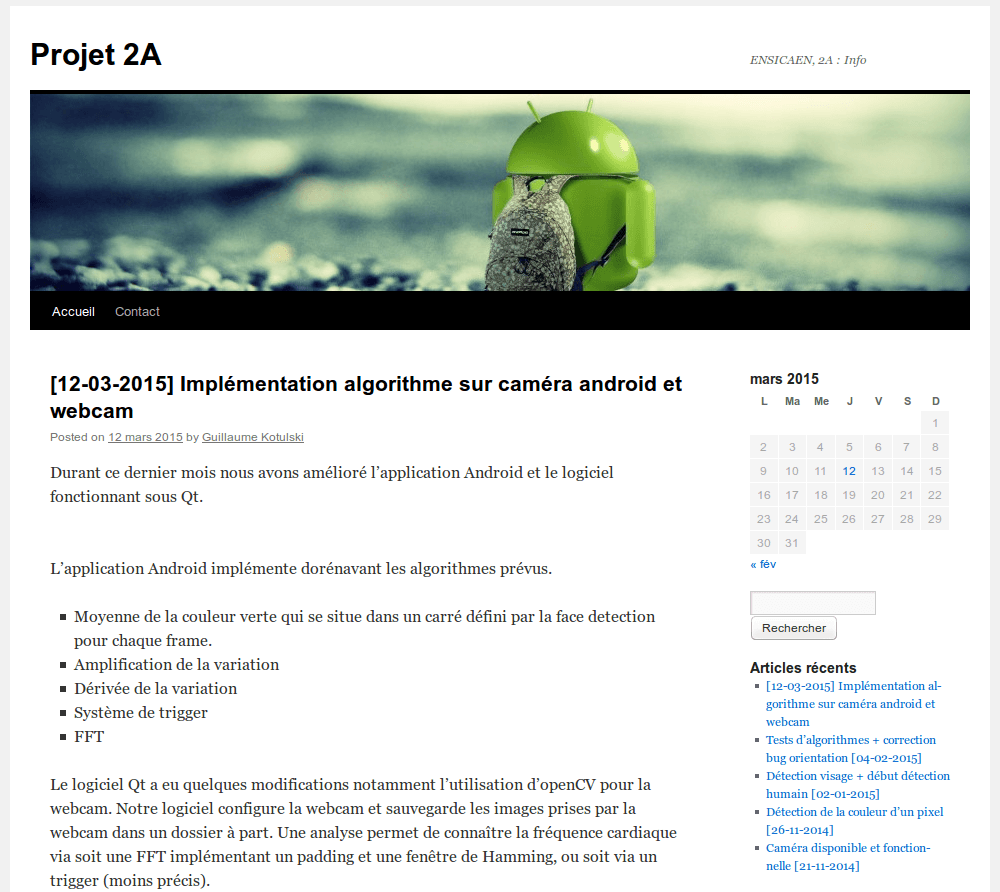
\includegraphics[width=0.9\textwidth]{data/website.png}
			\caption{Capture d'écran du site web.}
		\end{figure}

	\item Afin de partager le code source entre nous, nous avons utilisé le gestionnaire de versions Git :
		\begin{itemize}[label=\textbullet]
			\item Application Android: \url{https://github.com/F4r3n/Vamp}
			\item Logiciel de traitement d'images: \url{https://github.com/F4r3n/ImageProject.git}
		\end{itemize}
	\item Enfin, pour pouvoir avoir une vue globale sur les tâches à réalisées, en cours et déjà faites, nous avons utilisé le gestionnaire de projets Trello.
\end{itemize}

\section{Technologies utilisées}

\begin{itemize}[label=\textbullet]
	\item Qt : Nous avons utilisé la librairie Qt pour pouvoir créer notre application qui permettait de tester les algorithmes.
	\item Android : La programmation sous Android s'est faite en utilisant le Java et de l'XML\footnote{Extensible Markup Language}.
	\item OpenCV : Utilisation de la webcam et application utilisant la caméra gérée par OpenCV\footnote{Open Computer Vision}
	\item Python : Traitement des données pour création d'un graphique et permet une meilleure vérification des résultats
\end{itemize}

\section{Algorithme mis en place}

L’\oe il humain est limité, en effet il est incapable de voir les subtils changements temporels. Alors qu'au contraire en effectuant des traitements sur une vidéo, on est capable de
 révéler ces changements comme par exemple, la circulation du sang. Le sang parcourt notre corps de haut en bas de manière perpetuelle, ce mouvement imperceptible pour un oeil humain peut
 être capturée par notre téléphone portable. En travaillant sur ces infimes changements, on peut même grâce à ça réussir à connaître le pouls d'une personne. Mais comment obtenir ces
  changements ? Comment savoir où se situe le visage ?\\

Dans un premier temps, nous devons arriver à détecter la présence d'un visage humain devant l'appareil, en utilisant l'api de Google et même la libraire d'OpenCV, cela se fait bien.
Grâce à cette détection, nous pouvons obtenir les coordonnées du visage détéctées.\\

Maintenant que nous savons où se situe le visage, nous nous demandons comment reconnaître une fréquence ?\\

 \subsection{Choix de l'espace de couleur}
 Le choix de l'espace de couleur est primordial. C'est en fonction de celui-ci que nous obtiendrons des résultats cohérents ou non.\\
 Un des points important à prendre en compte fut le changement de luminosité, en se placant dans les espaces HSV\footnote{Hue Saturation Value}, HSL\footnote{Hue Saturation Lightness} ou YUV et en ne sélectionnant que les canaux Hue et Saturation par exemple pour HSV. Nous
  pensions obtenir des résultats ne dépendant pas de la luminosité. Sauf que les résultats obtenus par ces espaces de couleur n'étaient pas cohérents.\\
 \\
 Le second espace de couleur choisit fut RGB\footnote{Red Green Blue}, en effet même si celui-ci dépend fortement de la luminosité, nos résultats étaient meilleurs. Nous pouvions visualiser plus efficacement les changements de
 variation avec une dérivée.\\
 \\
 Après le choix de cet espace de couleur nous devions voir quel canal permetterait d'obtenir des variations les plus fortes. Pour ce faire nous avons visualisé les résultats de notre algorithme sur des personnes ayant des couleurs de peau différentes et avec les différents canaux (Red, Green, Blue). Nous remarquions que les résultats étaient meilleurs si nous utilisions seulement le canal Green.


 \subsection{Obtention des données}
 Nous avons donc fait une moyenne du canal vert (c'est le canal vert qui varie le plus) pour chaque pixel se situant dans un rectangle (en l’occurrence le rectangle délimitant le visage).
 Et ceci pour chaque frame que l'on capturait, nous obtenions une certaine valeur.\\
 Après obtention de ces valeurs, nous pouvions les traiter.\\\\
 La variation des valeurs étant très grande, nous avons dans un premier temps fait une moyenne glissante. Puis, pour amplifier les variations nous avons avons fait une dérivée de Taylor. \\Enfin nous filtrons les données grâce à un filtre passe-bas, pour diminuer le bruit en basse fréquence.
 Nos valeurs étant prêtes à être analysées, nous les avons traitées de deux façons différentes.\\
 La première, la plus simple fut le Trigger, qui nous permettait d'avoir une fourchette de pulsation.
 Le Trigger est une méthode permettant de connaître le nombre de fois qu'une fonction passe dans une bande de valeurs. Dans notre cas nous regardions combien de fois nous passions par 0 pour la dérivée.
 \\ La deuxième plus longue, une FFT\footnote{Fast Fourier Transform}, nécessitait des étapes de calcul supplémentaires telles qu'un fenêtrage de Hamming ou encore un padding, mais donnait des résultats plus précis.
 \\
 Ces deux analyses nous ont permis d'avoir le pouls de notre utilisateur (dans le cas idéal, c'est à dire lorsque la caméra et l'utilisateur ne bougeaient presque pas).
 \\\\

Nous avons remarqué que la collecte des données n'accentuait pas assez les variations, nous avons donc créé une deuxième méthode qui en restant basé sur le même principe que la première technique, nous découpions notre image
par zone de petits carrés de pixels. Par exemple une zone serait d'une taille de 5*5. On réalise ainsi une moyenne de chaque zone, puis par la suite une moyenne de ces moyennes. Enfin on rapplique les mêmes fonctions citées précédemment.

\begin{figure}[h!]
	\centering
	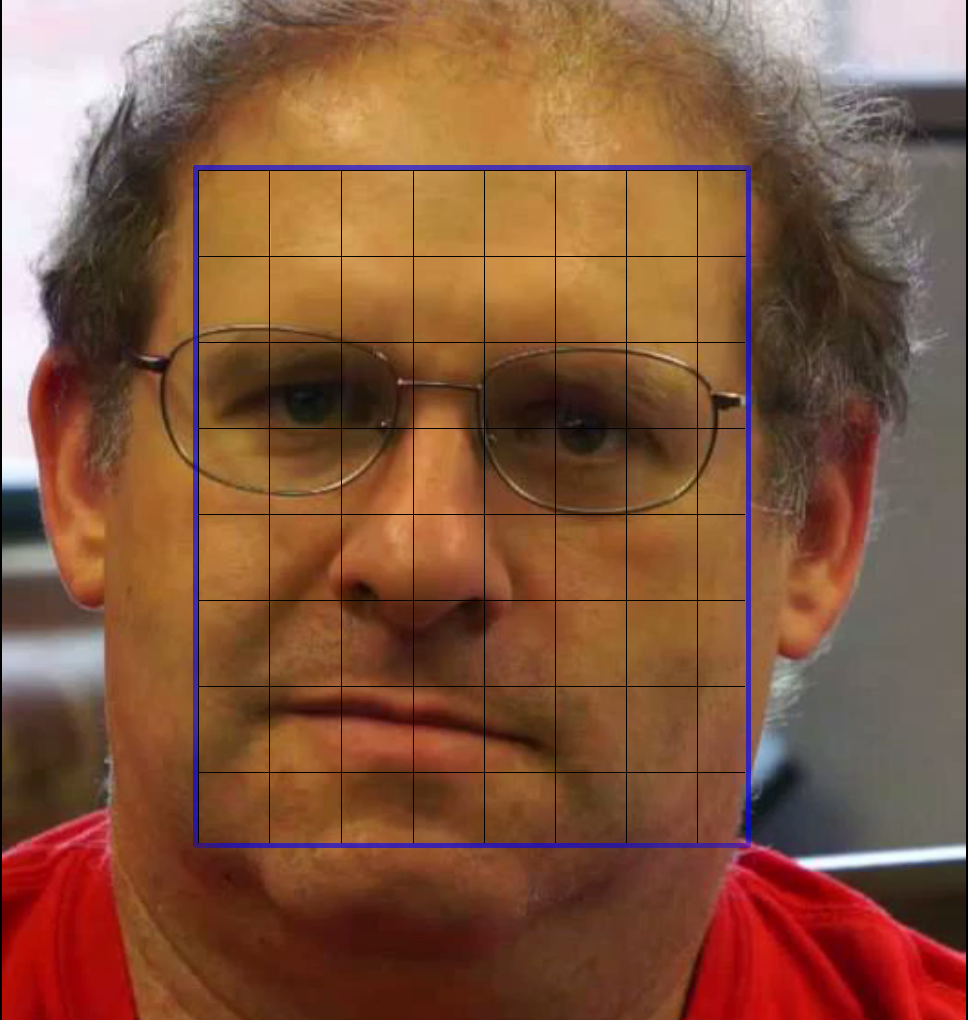
\includegraphics[width=0.5\textwidth]{data/algo-schema.png}
	\caption{Schéma de l'algo précédent}
\end{figure}


\section{Solutions mis en place}

Durant le projet nous avons développé plusieurs outils pour répondre au besoin. Une application Android qui permettrait d'utiliser le moyen d'authentification désiré et ainsi déverrouiller le smartphone d'une
personne. \\Un logiciel C++ utilisant la librairie Qt a également été mis en place, afin de pouvoir tester plus facilement les algorithmes que nous voulions développer. Dans la suite du projet, il a également
permis d'utiliser la webcam.

\subsection{Développement Android}

Notre application Android est capable d'utiliser la caméra frontale de n'importe quel smartphone. \\\\L'api d'Android propose une classe appelée \href{http://developer.android.com/reference/android/hardware/Camera.FaceDetectionListener.html}{FaceDetectionListener} qui va permettre de
 capter, les visages présent devant une caméra, grâce à ce système il est possible de dessiner un Rect (c'est à dire un rectangle) autour du visage de la personne.\\\\ C'est notre classe
  DisplayedFace qui se charge de ce travail.
Une fois la reconnaissance mis en place, nous avons utilisé la fonction
\href{http://developer.android.com/reference/android/hardware/Camera.PreviewCallback.html#onPreviewFrame\%28byte\%5B\%5D,\%20android.hardware.Camera\%29}{onPreviewFrame}. Cette dernière permet d'enregistrer
en temps réel, les données. On lance un compteur quand la première reconnaissance d'un visage a lieu, ce dernier va durer 5 secondes.\\

\begin{figure}[h!]
	\centering
	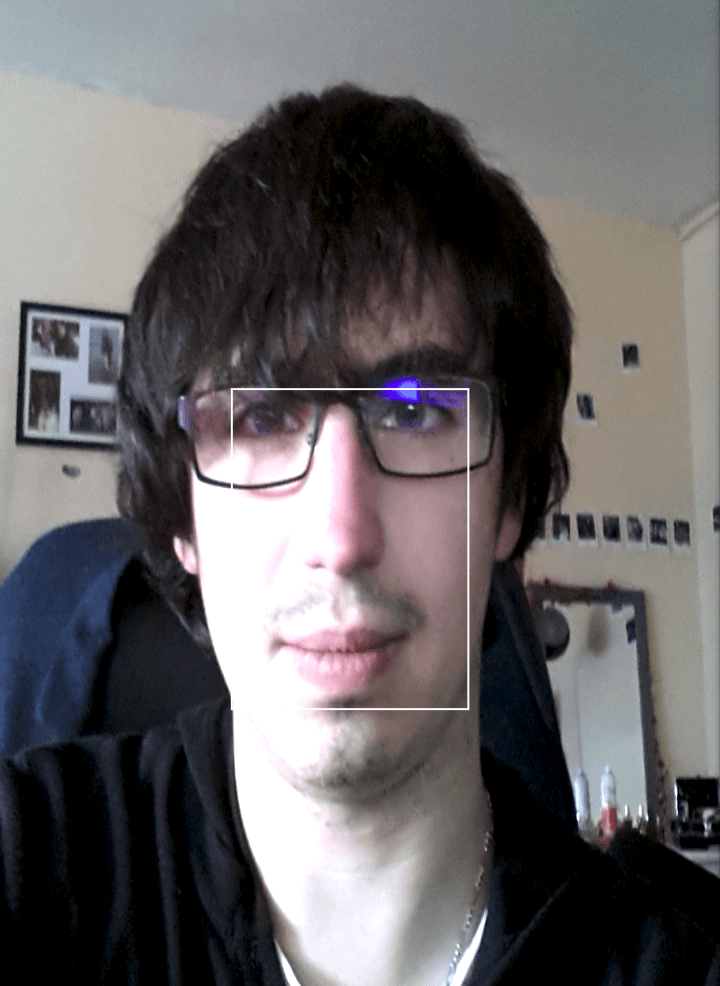
\includegraphics[width=0.5\textwidth]{data/appAndroid.png}
	\caption{Aperçu de l'application Android}
\end{figure}

Les données ainsi récoltées sont au format de l'espace de couleur \href{http://fr.wikipedia.org/wiki/YUV}{YUV}. Nous devons donc convertir ces données au format RGB qui se révèle plus évocateur au niveau des variations.\\\\

A la fin du compteur, on réalise une dérivée, puis une amplification des valeurs obtenues. On observe alors les variations qu'on obtient et on conclut alors sur la présence ou non d'un humain.\\
\\
L'api de Google est très rapide pour détecter un visage et pour nous fournir ces coordonnées en faisant très peu de calculs. Mais celle-ci ne suit pas les petits changements de position, par exemple lorsque l'utilisateur prend une vidéo il bouge légèrement ce qui peut changer le résultat final.\\
\\
Pour résoudre ce manque nous avons codé une application fonctionnant avec OpenCV, celle-ci suit parfaitement le visage lorsqu'il bouge. Mais le temps de traitement d'une image par OpenCV est beaucoup plus lent que l'api de Google. Nous tournons à environ 7 FPS\footnote{Frame Per Second} en utilisant la back-caméra et 2 FPS en utilisant la front-caméra, ce qui n'est pas idéal.
\begin{figure}[h!]
	\centering
	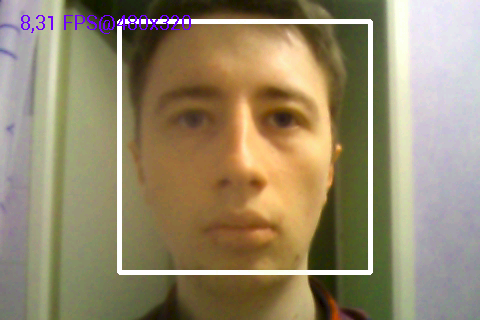
\includegraphics[width=0.8\textwidth]{data/opencv.png}
	\caption{Aperçu de l'application OpenCV}
\end{figure}
\\
\\
L'application sous OpenCV permet de faire une FFT et un système de Trigger, en croisant les résultats donnés par ces deux systèmes nous obtenons un meilleur résultat que s'il n'y avait que le Trigger.

\subsection{Développement C++}

Nous avons créé un logiciel C++ nous permettant de tester nos algorithmes avant de les implémenter sous Android.
Ce logiciel a de nombreuses fonctionnalités, notamment le découpage d'une vidéo en images pour permettre une analyse plus poussée.
Nous utilisons Avconv qui permet de découper une vidéo de n'importe quelle taille en une multitude d'images. (15 images * taille de la vidéo)
Après avoir découpé la vidéo en images nous faisons une analyse sur ces images.
Cette analyse se découpe en plusieurs étapes.\\\\

Dans un premier temps nous dessinons un rectangle autour d'un visage (si la fonction du rectangle automatique n'est pas enclenchée).
Puis nous choisissons le type d'analyse à effectuer, il y en a deux types:
\begin{itemize}
	\item L'une fait la moyenne de tous les pixels qui se situe dans le carré
	\item La seconde découpe le rectangle en plusieurs zones de 5*5 puis amplifie les variations et fait une moyenne des valeurs
\end{itemize}
Après avoir lancé l'analyse, nous affichons les courbes ainsi obtenues par notre application.\\\\

Nous pouvons voir la FFT, l'amplification, la dérivée ou une combinaison de plusieurs méthodes.
L'amplification utilise la dérivée de Taylor du premier degré.
La FFT utilise un filtre passe-bas combiné avec une fenêtre de Hamming et un padding.
La FFT permet de connaître le rythme cardiaque d'une personne de manière précise si l'image est assez stable.
Nous avons créé un Trigger qui permet aussi de connaître la fréquence cardiaque d'une personne, mais de manière moins précise, le Trigger nous donne une fourchette de valeurs.\\\\

Si l'espace de couleur que nous avons choisi ne donne pas des résultats corrects nous pouvons en choisir un autre.
Nous avons différents espaces de couleur disponibles dont RGB, HSL, HUV et nous pouvons lancer une analyse avec un espace de couleur différent de RGB.\\\\

Les analyses avec des vidéos classiques n'étant pas suffisantes pour nos tests, nous avons dû faire une analyse avec des vidéos de la webcam.
La webcam est configurée et lancée via la librairie OpenCV et nous enregistrons les images de la webcam avec une fréquence de 15 frames pas seconde.\\\\

\section{Problèmes rencontrés}

\subsection{Limitation des sessions à l'ENSICAEN}

Lors du projet, nous avons rencontré de nombreux problèmes. L'un des plus embêtants fut la limite des sessions à l'Ensicaen. En effet, nos sessions disposent d'une taille limitée, nous
 pouvons uniquement travailler sous Windows (car c'est seulement sous cet environnement que sont installés les outils Android) hors nous disposons d'uniquement 150 Mo, or rien qu'avec
  Firefox, si nous ne nettoyons pas régulièrement l'historique, la session se retrouve complète. Nous avons malheureusement expérimenté le souci et perdu ainsi, une après-midi de travail.

\subsection{Problèmes rencontrés lors du développement Android}

Nous avons eu un problème de rotation, les coordonnées que l'on conversaient se révélaient mauvaise. Afin d'éviter cela, nous avons décidé de forcer le mode portrait.

La première version de notre application était capable d'enregistrer 15 frames par seconde, or au final on obtenait seulement une trentaine de valeurs, cela était dû à la conversion du
 format YUV au format RGB que l'on effectuait à chaque fois que nous rentrions dans la fonction onPreviewFrame, comme la conversion est coûteuse O(n\up{2}), on perdait des valeurs. Pour
  optimiser, le nombre de valeurs nous effectuons maintenant la conversion une fois le timer fini. On réalise alors dans la boucle une simple sauvegarde des données brutes.
Toutefois cette méthode, nous a causé pas mal de soucis, notamment des out of memory, c'est-à-dire, que nous réalisions une allocation trop importante par rapport à la mémoire disponible
\ldots{}\\
\\
Même si l'algorithme fonctionnait avec des vidéos, ceci ne voulait pas dire qu'il fonctionnerait sous Android. En effet lorsque avec la caméra on se prend en vidéo on bouge légèrement,
ce qui pose de nombreux problèmes de stabilité. Les variations que nous obtenions alors ne seraient plus celle de la pulsation mais celles du mouvement régulier de la main.


\chapter{Résultats}
\section{Cadre idéal}

\subsection{Définition du cadre idéal}
Notre algorithme fonctionne parfaitement dans le cadre idéal, une fois sortie de ce cadre les résultats sont moins précis et peuvent être incohérents. \\Ayant choisi un espace de couleur RGB, le moindre changement de luminosité nous donne des résultats in cohérents. \\\\
Il faut que l'appareil tel que la webcam ou le smartphone ne bouge pas lors de la collecte des données. Si celui-ci bouge de trop nous allons détecter des variations et notre application la percevra comme des fréquneces cardiaques.\\\\
L'appareil doit enregistrer les données avec une résolution supérieure à 480*320.\\
La personne filmée ne doit être pas trop éloignée de l'objectif pour avoir des résultats optimaux.

\subsection{Résultats dans le cadre idéal}
Nous avons effectué différents tests durant le projet. En utilisant les vidéos fournies sur le site dû MIT\@. Notre logiciel arrive à obtenir des 
résultats très correct. En effet, par exemple comme on peut le voir sur cette capture d'écran. Après notre magnification réalisée, on retrouve
une fréquence cardiaque d'environ 53 battements par minute (BPM), l'article du MIT lui trouve une fréquence de 54 BPM\@. 

\begin{figure}[h!]
	\centering
	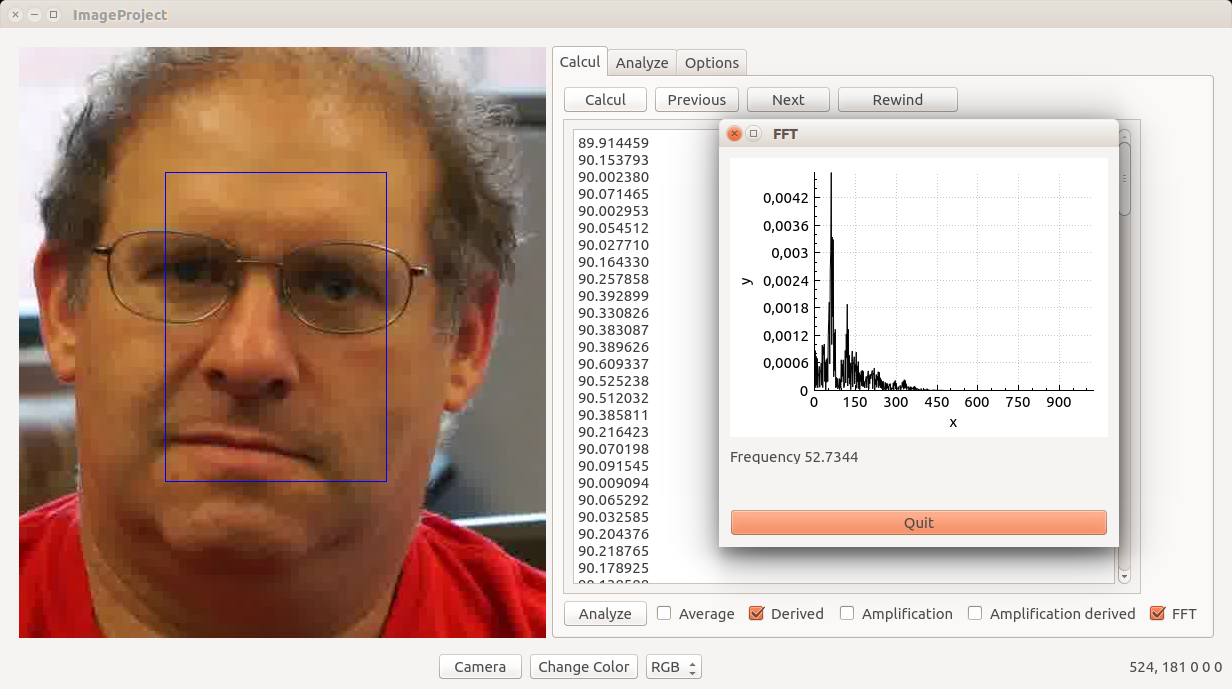
\includegraphics[width=0.9\textwidth]{data/cas-ideal.png}
	\caption{Vidéo source du MIT analysé avec notre logiciel.}
\end{figure}

On pouvait se poser la question, des personnes de couleur, est-ce qu'une couleur de peau différente aurait pu avoir des conséquences? Nous avons
donc tester avec une autre vidéo fournie par le MIT avec une personne de peau noir, on peut voir sur la capture suivante que cela n'a en rien influencer
sur notre algorithme. On retrouve donc une fréquence comprise entre 47 et 59 BPM\@.

\begin{figure}[h!]
	\centering
	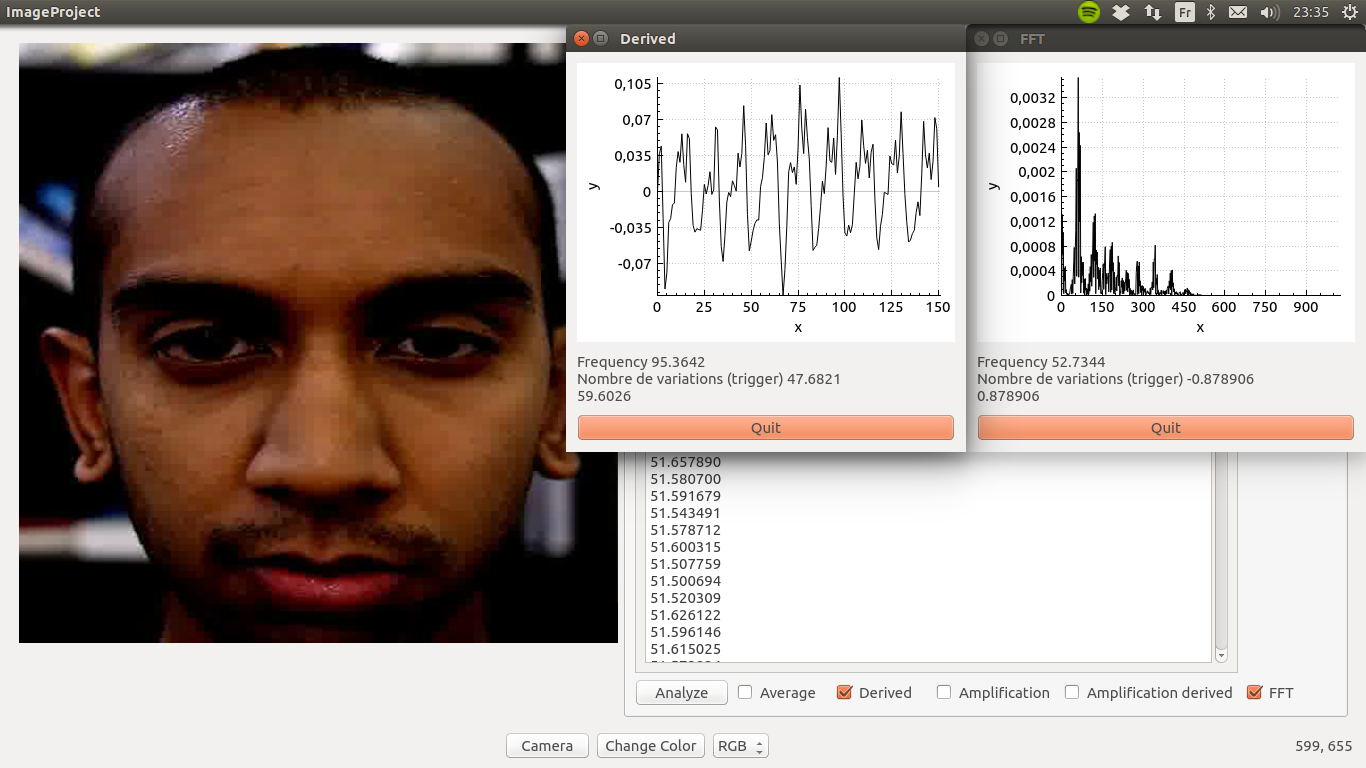
\includegraphics[width=0.9\textwidth]{data/logi.png}
	\caption{Autres test avec une personne de couleur de peau différente.}
\end{figure}


\section{Webcam}

Avec une webcam, nos résultats sont moins précis, mais sont assez correct pour être utiliser. 

\begin{figure}[h!]
	\centering
	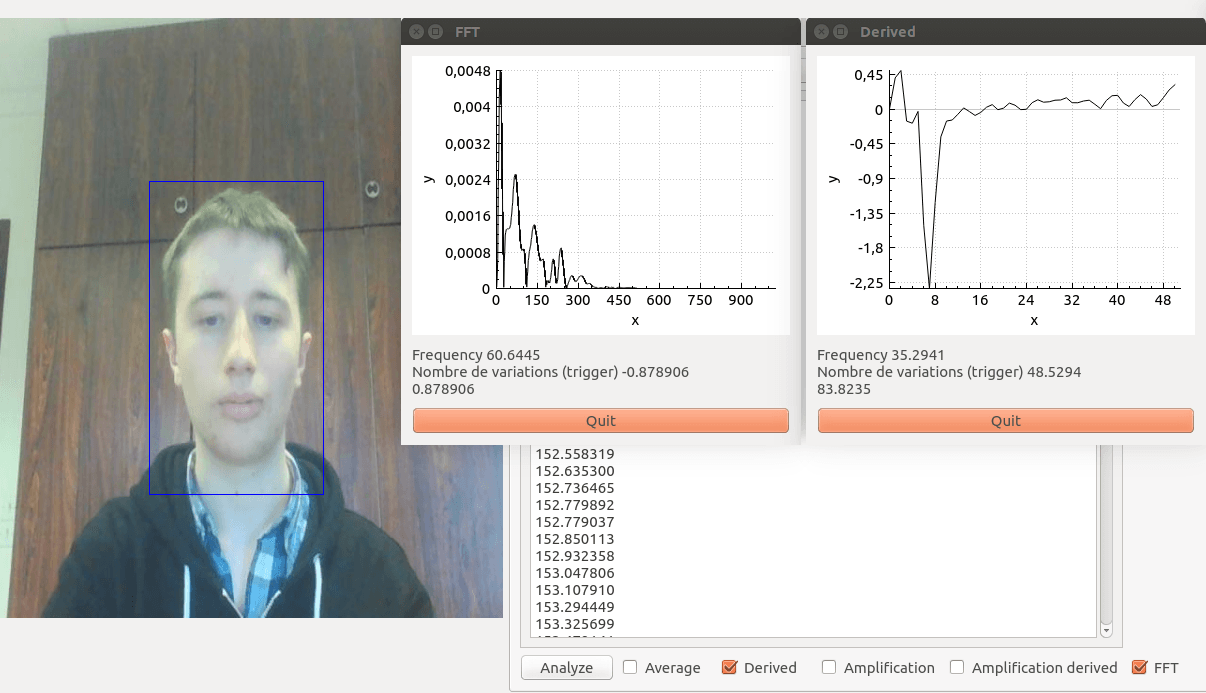
\includegraphics[width=1\textwidth]{data/webcam.png}
	\caption{Vidéo pris par la webcam et analysé avec notre logiciel.}
\end{figure}

\section{Mobile}

\subsection{Android}

Notre plus gros problème a était lors de nos tests sur Android, la stabilité de la vidéo et le nombre de frames capturés.
Actuellement notre application est capable de capturer des frames et appliquer notre algorithme mais nos résultats restent erronées.

\subsection{OpenCV}
L'utilisation d'une FFT et d'un Trigger permet de mieux différencier l'homme de la photo. Même si les résultats sont meilleurs il reste de nombreuses erreurs et le temps de calcul est beaucoup plus long.

\subsection{Ressources utilisées}
La mémoire accordé à notre application par le système d'exploitation de l'ordinateur est fixe et ne peut être augmenté.\\
Donc nous devons faire nos enregistements avec une mémoire limitée, c'est à dire que le nombre d'image capturée était limité. Une plus grand resolution de la caméra implique donc moins d'images à enregistrer. \\
De plus le nombre d'opération a effectué étant important, nous avions un temps de calcul assez important sous OpenCV\@. Pour 10 secondes d'enregistement avec une résolution de 480*320 à raison de 6 images par seconde, soit 60 images nous obtenions un temps de calcul de 20 secondes. Ce qui es beaucoup trop important pour une application qui se veut rapide.\\
Sous android natif le problème fut que le nombre d'images capturé n'était pas suffisant pour permettre une analyse correcte, un enregistement d'un nombre trop important d'image (supérieur à 30) engendrait un crash de notre application.



\section{Bilan}

Notre différenciation entre un humain et une photo fonctionne correctement dès lors où la stabilité est assurée. En effet, prenons Android, nous arrivons
à capturer plus de frames qu'en utilisant OpenCV, toutefois le tracking d'OpenCV est plus efficace. De ce fait, malgré une meilleure capture sous Android 
comme la stabilité est plus mauvaise, nos résultats sont moins bons. Mais à contrario, lorsqu'on utilise l'application réalisée avec OpenCV, le nombre d'images
capturé est seulement de 20 pour 4 secondes, avec si peu d'images à traiter notre magnification n'est pas correcte. C'est seulement au bout de 10 secondes
lorsqu'on capture entre 50 à 70 frames qu'on a des résultats cohérents. 



\chapter{Conclusion}
\section{Apports techniques}

Ce projet nous a permis de mettre en œuvre l'enseignement que nous a donné l'ENSICAEN, l'utilisation de Github, les cours de Java/C++ et de conception d'interface graphique. Il nous a également permis d'
apprendre le développement mobile et l'utilisation de librairie comme OpenCV\@.

\subsection{Android}
	Android est un système d'exploitation sur lequel nous n'avions jamais programmé, l'appréhender par nous même fut difficile.
	Le placement des widgets sur l'écran et même le système d'activité, nous étaient inconnus et nous avions passé de nombreuses heures à le comprendre complètement.
	De plus notre projet utilse la caméra, l'un des périphériques, le plus difficile à mettre en place.

	L'un des plus gros avantages d'android, c'est la documentation qui est bien écrite, ce qui est très appréciable. Grâce à ce projet, nous avons pu avoir un aperçu du système, de ces forces et
	de ces faiblesses.

\subsection{Qt}
	Nous avons déjà eu quelques expériences avec cette bibliothèque, mais nous avons réellement pu appliquer nos connaissances avec ce projet.
	Notre logiciel de test fut d'une grande aide pour l'intégration de nos algorithmes sous Android.\\
	Ce logiciel comprenant de nombreux modules, nous avons dû appliquer des méthodes vue en génie logiciel pour que celui-ci fonctionne correctement.

\subsection{OpenCV}
Nous avons dû utiliser la bibliothèque OpenCV, ce qui était une nouveauté. Celle ci nous a permis d'avoir un meilleur contrôle des images prises par la webcam.

\section{Apports scientifiques}

Nous avons également pu mettre à profit les cours que nous avons eus sur les différents espaces de couleurs, surtout utiles comme nous l'avons vu lors du développement Android.
Le plus gros défi fut la mise en place de techniques du traitement du signal, telle que la FFT ou encore la réalisation d'un filtre basse fréquence.

\section{Bilan}

Ce projet a donc été un vrai aboutissement de notre formation. Il nous a forcé à appréhender de nouvelles technologies et librairies mais également à réutiliser tout ce que nous
 connaissions. Nous avons pu voir les nombreux avantages d'une documentation bien construite et bien imagée, cela permettant de bien sur s'approprier rapidement la technologie étudiée.


\appendix
\chapter{Annexes}
Voici l'article du MIT sur la magnification d'une vidéo, nous avons choisi
de prendre juste le début du billet car il correspond à leur développement 
sur la couleur, la partie sur laquelle nous avons travaillés.

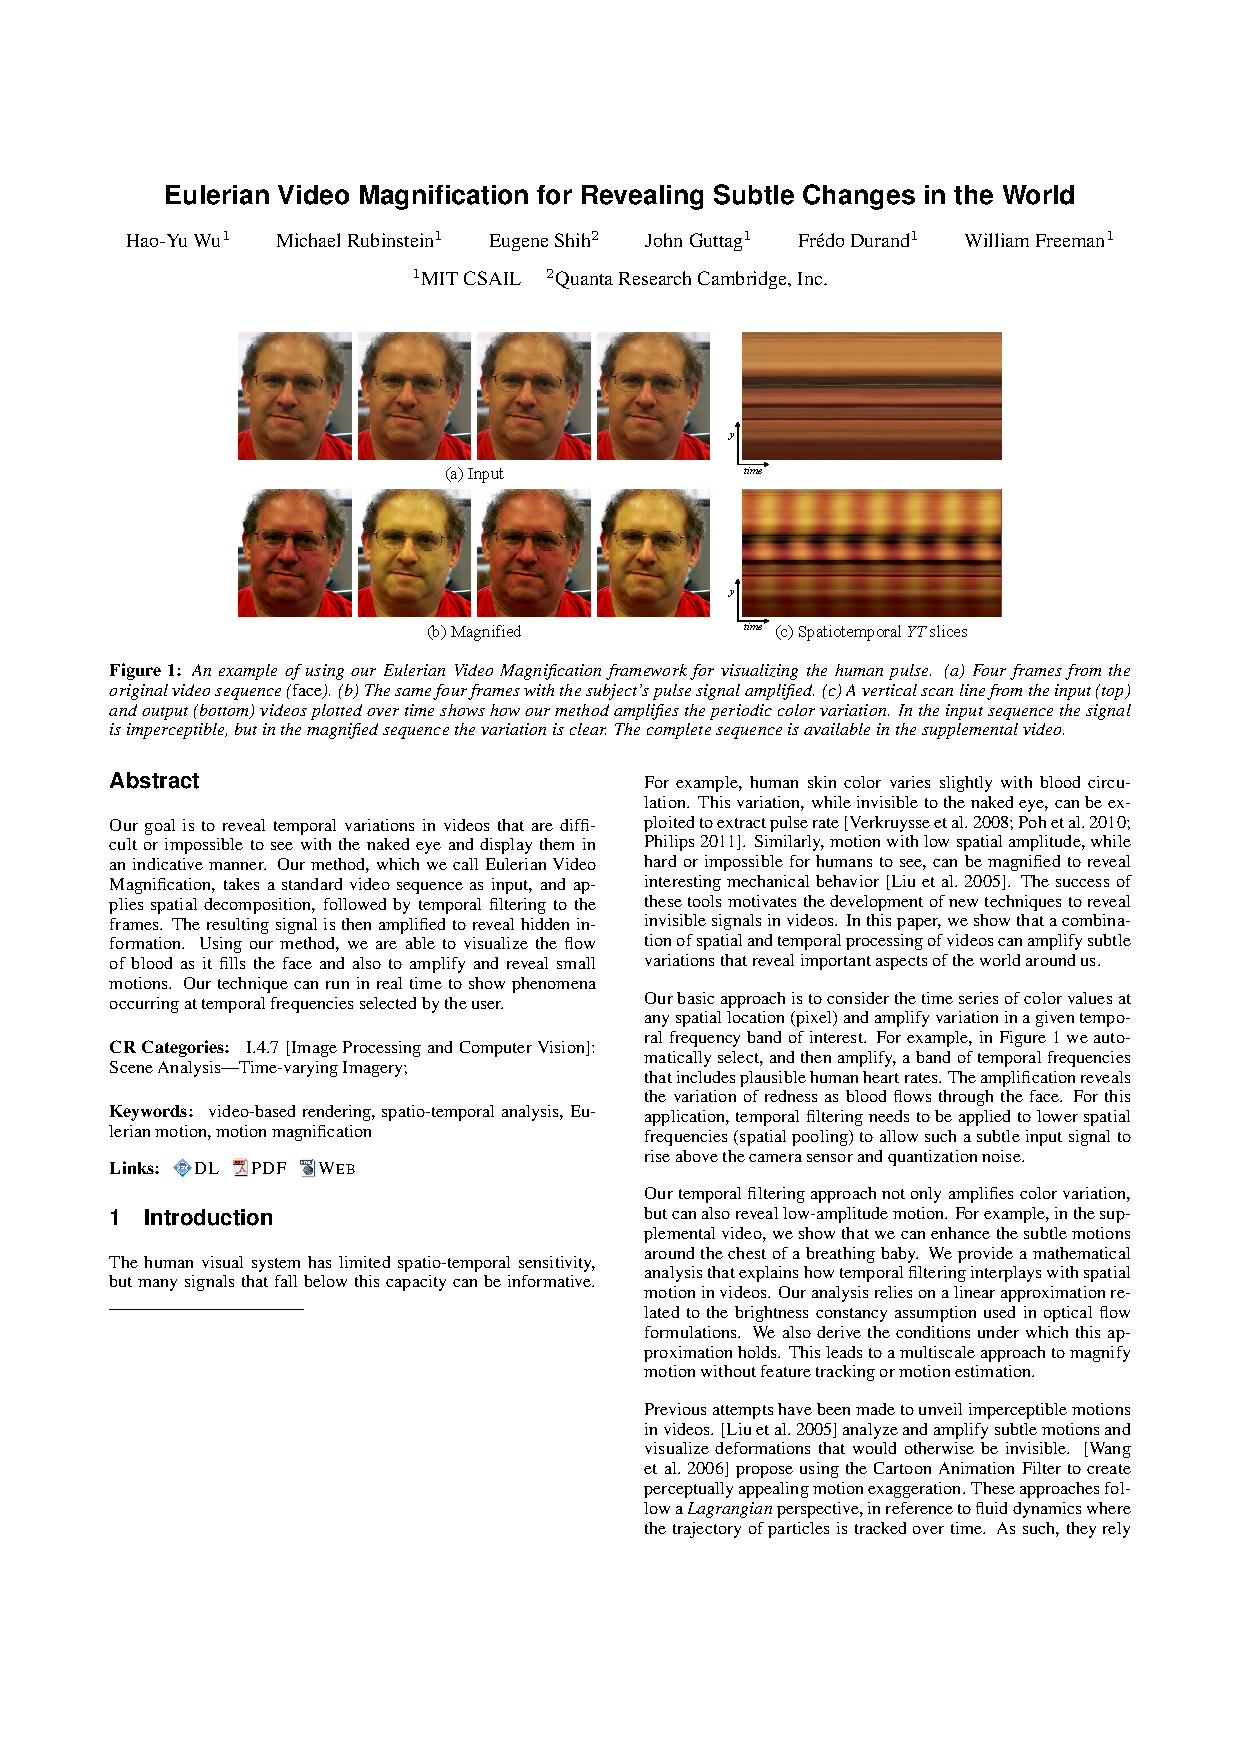
\includepdf[pages=-]{data/annexes.pdf}


\end{document}
